%
% d.tex -- slide template
%
% (c) 2021 Prof Dr Andreas Müller, OST Ostschweizer Fachhochschule
%
\bgroup
\begin{frame}[t]
\setlength{\abovedisplayskip}{5pt}
\setlength{\belowdisplayskip}{5pt}
\frametitle{Diedergruppen}
\vspace{-20pt}
\begin{columns}[t,onlytextwidth]
\begin{column}{0.33\textwidth}
\begin{block}{$D_n$}
\begin{center}
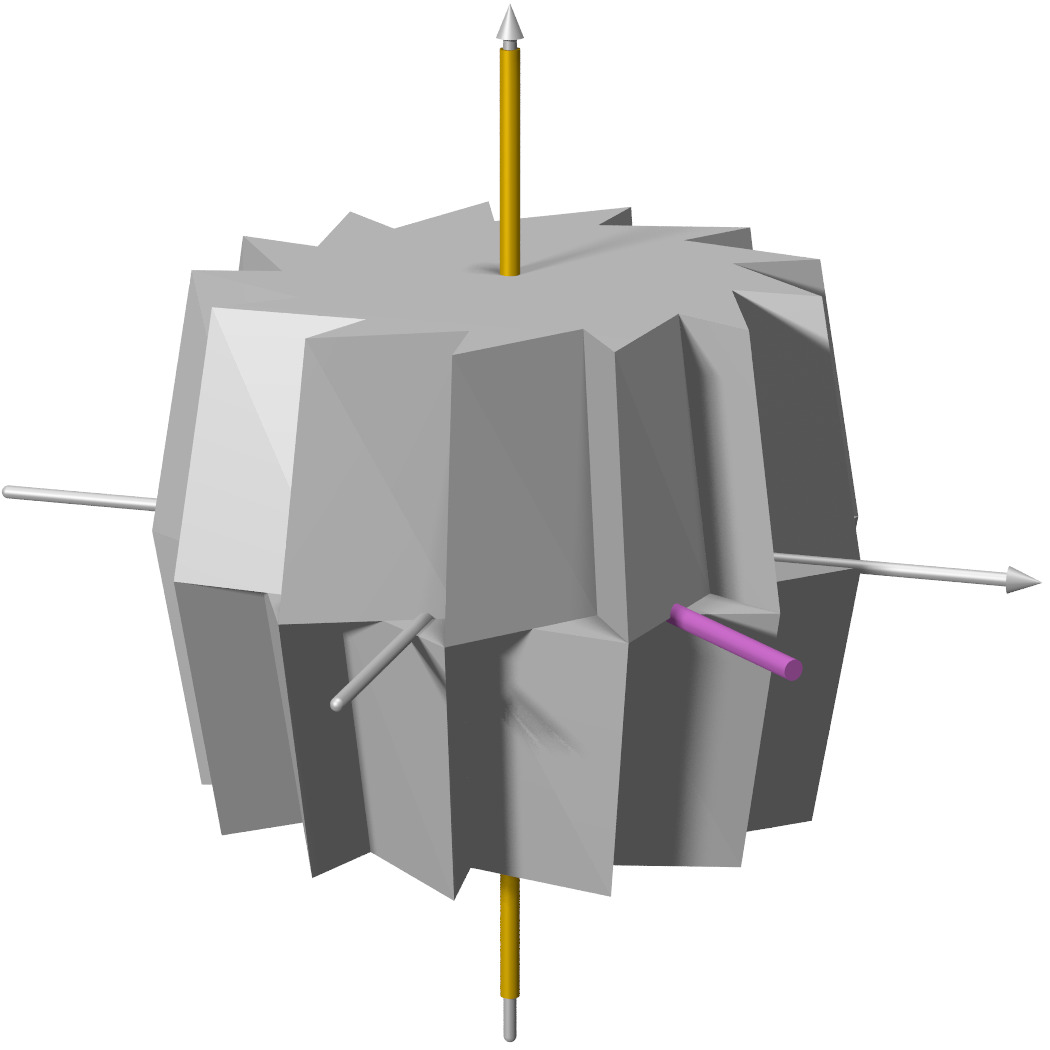
\includegraphics[width=\textwidth]{../slides/6/punktgruppen/images/dn.jpg}
\end{center}
\vspace{-8pt}
\begin{itemize}
\item $C_n$ Achse
\item $n$ $C_2$ Achse senkrecht dazu
\end{itemize}
\end{block}
\end{column}
\begin{column}{0.33\textwidth}
\uncover<2->{%
\begin{block}{$D_{nd}$}
\begin{center}
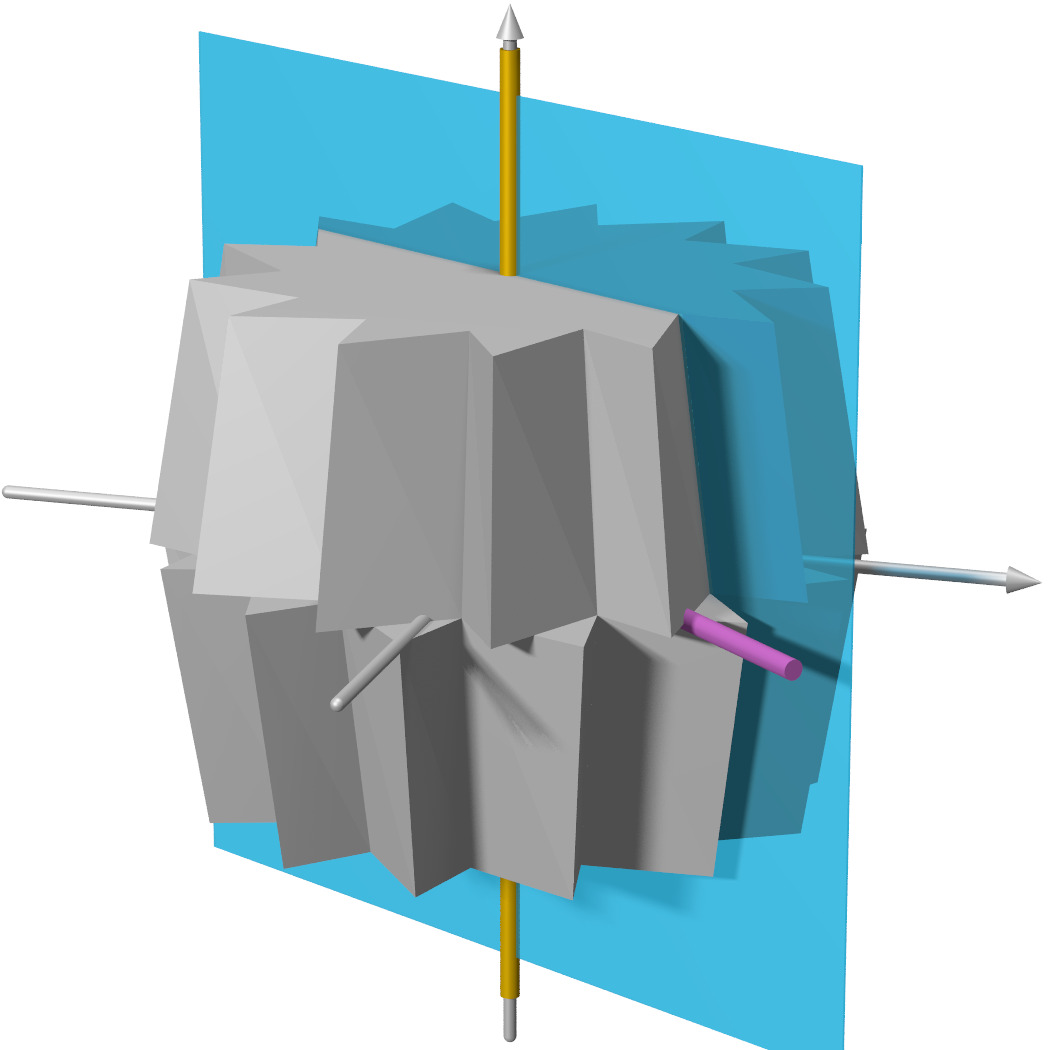
\includegraphics[width=\textwidth]{../slides/6/punktgruppen/images/dnd.jpg}
\end{center}
\vspace{-8pt}
\begin{itemize}
\item $D_n$ Achse
\item $n$ winkelhalbierende Spiegelebenen der $C_2$-Achsen
\end{itemize}
\end{block}}
\end{column}
\begin{column}{0.33\textwidth}
\uncover<3->{%
\begin{block}{$D_{nh}$}
\begin{center}
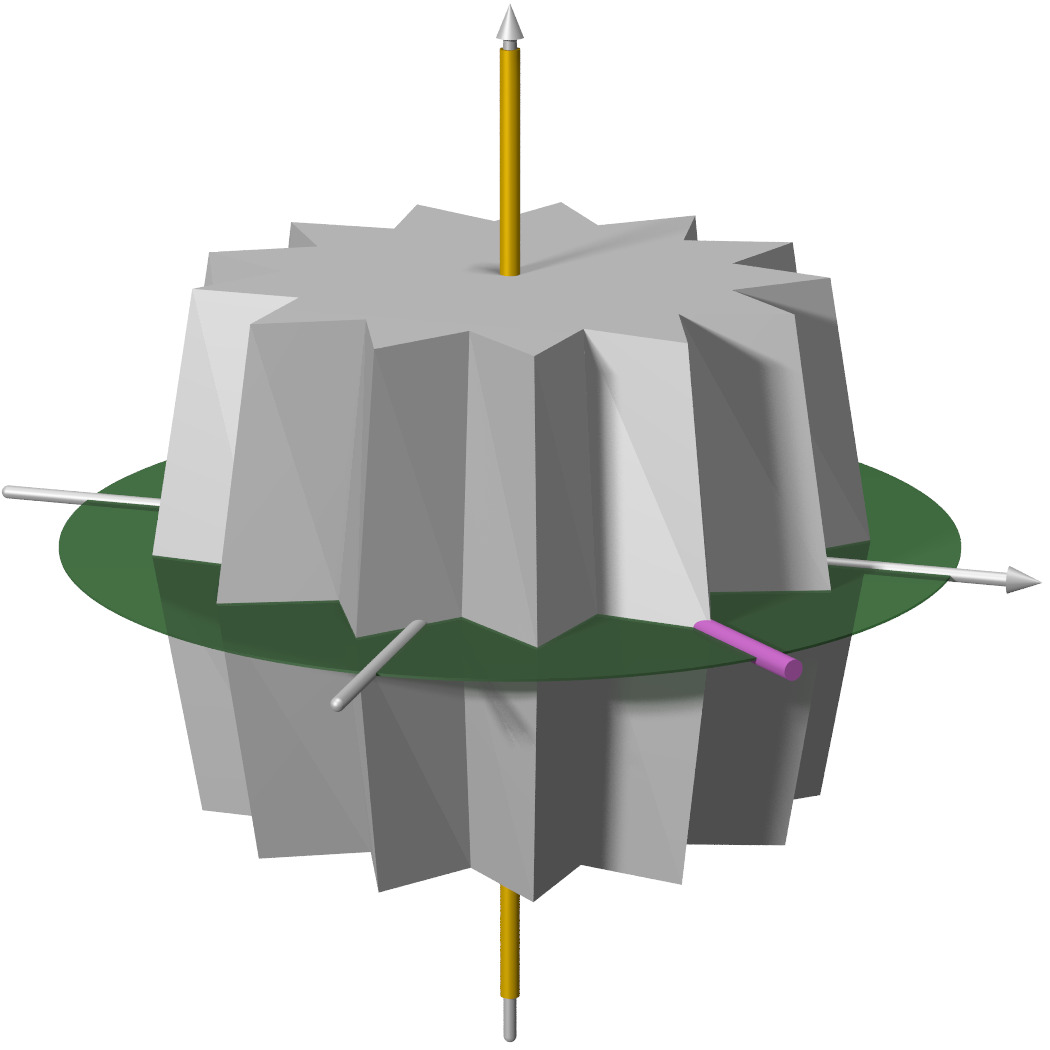
\includegraphics[width=\textwidth]{../slides/6/punktgruppen/images/dnh.jpg}
\end{center}
\vspace{-8pt}
\begin{itemize}
\item $D_n$ Achse
\item Spiegelbene senkrecht dazu
\end{itemize}
\end{block}}
\end{column}
\end{columns}
\end{frame}
\egroup
